\chapter{Diseño de la solución propuesta} \label{chap:3}

Este capítulo tiene como objetivo, describir la propuesta para la importación de los datos provenientes de un fichero, en datos que gestiona la herramienta TEAMSOFT$^+$. Para lograr esto, se muestran los artefactos de ingeniería de software necesarios para entender su funcionamiento, como son: diagrama de casos de uso del sistema y diagrama de paquetes. Además se realiza la validación de la solución propuesta.

\section{Artefactos de ingeniería de software}

En esta sección se muestran los artefactos de ingeniería de software necesarios para entender y explicar el funcionamiento de la funcionalidad de importar el fichero.

\subsection{Diagrama de casos de uso}

La funcionalidad a incorporar se relaciona con la inserción de nuevas personas personas, competencias y roles. Es por este motivo que se decide que el responsable de llevarlas a cabo sea el rol \textbf{Gestor de recursos humanos}. Debido a la gran número de CU que posee el sistema, se decide mostrar solamente los aquellos que fueron modificados o creados por el autor. En la Figura \ref{fig:CU_nuevo} se muestra el diagrama el diagrama de CU correspondiente. El color verde corresponde a los CU no modificados, el amarillo a los modificados y el color rojo corresponde a los CU incorporados.

\begin{figure}[H]
	\centering
	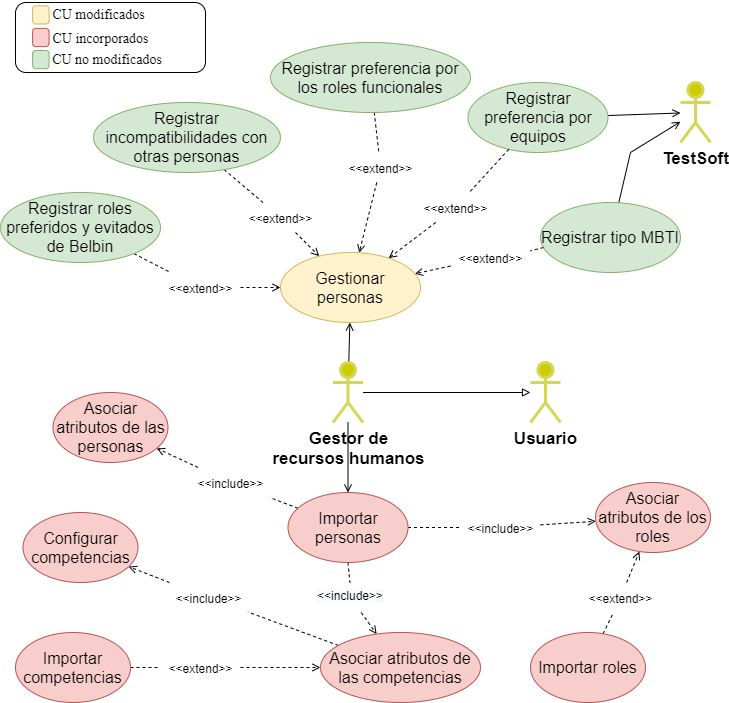
\includegraphics[width=\textwidth]{figuras/diagrama_CUTeamSoftImportar.png}
	\caption{Ampliación de diagrama de CU} \label{fig:CU_nuevo}
\end{figure}
	
\subsection{Descripción de alto nivel de los casos de uso}
En esta sección se describen cada uno de los casos de uso relacionadas con la funcionalidad a implementar. En cada uno se explican elementos tales como: el nombre, la descripción y los casos de uso relacionados.\\\\

La Tabla \ref{table:descripcion-alto-nivel-importar} muestra la descripción de alto nivel del CU Importar Personas.

\begin{table}[H]
	\centering
	\caption{Descripción de alto nivel del CU Importar Persona} \label{table:descripcion-alto-nivel-importar}
	\begin{tabular}{ | l | p{10cm} |}
		\toprule
		Nombre & Importar Personas \\ \midrule
		Descripción & Este es el CU principal del la funcionalidad propuesta. Para importar las personas el usuario debe seleccionar la opción de importar, luego el sistema le muestra una ventana donde debe localizar el archivo que desea importar. Si el fichero posee las características correctas se procede a leer el fichero. Además debe seleccionar (o crear) un grupo al cual asociar las personas a importar.\\ \hline
		CU relacionados & Asociar atributos de las personas, Asociar atributos de las competencias, Asociar atributos de los roles.\\ \bottomrule
	\end{tabular}
\end{table}

La Tabla \ref{table:descripcion-alto-nivel-atr-pers} muestra la descripción de alto nivel del CU Asociar atributos de las personas.

\begin{table}[H]
	\centering
	\caption{Descripción de alto nivel del CU Asociar atributos de las personas} \label{table:descripcion-alto-nivel-atr-pers}
	\begin{tabular}{ | l | p{10cm} |}
		\toprule
		Nombre          & Asociar atributos de las personas                                                                                                                                                \\ \midrule
		Descripción     & En este CU el usuario debe asociar de los atributos del fichero seleccionado, qué elementos corresponden con la experiencia y el nombre de las personas. \\ \hline
		CU relacionados &  \\ \bottomrule
	\end{tabular}
\end{table}

La Tabla \ref{table:descripcion-alto-nivel-atr-comp} muestra la descripción de alto nivel del CU Asociar atributos de las competencias.

\begin{table}[H]
	\centering
	\caption{Descripción de alto nivel del CU Asociar atributos de las competencias} \label{table:descripcion-alto-nivel-atr-comp}
	\scalebox{0.97}{
	\begin{tabular}{ | l | p{10cm} |}
		\toprule
		Nombre          & Asociar atributos de las competencias                                                                                                                                                \\ \midrule
		Descripción     & En este CU el usuario debe asociar a los atributos del fichero que tengan relación con las competencias. Debe especificar todas las competencias que se pueden calcular utilizando este atributo. \\ \hline
		CU relacionados &   Configurar competencias, Importar competencias \\ \bottomrule
	\end{tabular}
}
\end{table}


La Tabla \ref{table:descripcion-alto-nivel-conf-comp} muestra la descripción de alto nivel del CU Configurar competencias.

\begin{table}[H]
	\centering
	\caption{Descripción de alto nivel del CU Configurar competencias} \label{table:descripcion-alto-nivel-conf-comp}
	\scalebox{0.97}{
	\begin{tabular}{ | l | p{10cm} |}
		\toprule
		Nombre          & Configurar competencias                                                                                                                               \\ \midrule
		Descripción     & En este CU el usuario debe configurar los valores de los atributos relacionados con las competencias. Para esto el usuario debe establecerle a aquellos atributos que contienen campos de texto un valor entre 0 y 1. Un proceso similar debe realizar con aquellos atributos que tienen relación con las mismas competencias. Mientras que para aquellos atributos que almacenan valores numéricos, debe seleccionar el mayor valor presente en el fichero. \\ \hline
		CU relacionados &  \\ \bottomrule
	\end{tabular}
}
\end{table}

La Tabla \ref{table:descripcion-alto-nivel-imp-comp} muestra la descripción de alto nivel del CU Importar competencias.

\begin{table}[H]
	\centering
	\caption{Descripción de alto nivel del CU Configurar competencias} \label{table:descripcion-alto-nivel-imp-comp}
	\scalebox{0.97}{
	\begin{tabular}{ | l | p{10cm} |}
		\toprule
		Nombre          & Importar competencias                                                                                                                          \\ \midrule
		Descripción     &  Para importar las competencias el usuario debe seleccionar la opción de importar, luego el sistema le muestra una ventana donde debe localizar el archivo que desea importar. Si el fichero posee las características correctas se procede a leer el fichero.\\ \hline
		CU relacionados &  \\ \bottomrule
	\end{tabular}
}
\end{table}

La Tabla \ref{table:descripcion-alto-nivel-atr-role} muestra la descripción de alto nivel del CU Asociar atributos de los roles.

\begin{table}[H]
	\centering
	\caption{Descripción de alto nivel del CU Asociar atributos de los roles} \label{table:descripcion-alto-nivel-atr-role}
	\scalebox{0.97}{
		\begin{tabular}{ | l | p{10cm} |}
			\toprule
			Nombre          & Asociar atributos de los roles                                                                                                                              \\ \midrule
			Descripción     & En este CU el usuario debe asociar aquellos atributos del fichero que tengan relación con los roles. Debe especificar para cada atributo seleccionado el rol que le corresponde. \\ \hline
			CU relacionados & Importar roles \\ \bottomrule
		\end{tabular}
	}
\end{table}


La Tabla \ref{table:descripcion-alto-nivel-imp-role} muestra la descripción de alto nivel del CU Importar roles.

\begin{table}[H]
	\centering
	\caption{Descripción de alto nivel del CU Importar roles} \label{table:descripcion-alto-nivel-imp-role}
	\scalebox{0.97}{
		\begin{tabular}{ | l | p{10cm} |}
			\toprule
			Nombre          & Importar competencias                                                                                                                          \\ \midrule
			Descripción     &  Para importar los roles el usuario debe seleccionar la opción de importar, luego el sistema le muestra una ventana donde debe localizar el archivo que desea importar. Si el fichero posee las características correctas se procede a leer el fichero.\\ \hline
			CU relacionados &  \\ \bottomrule
		\end{tabular}
	}
\end{table}

La Tabla \ref{table:descripcion-alto-nivel-gestion-personas} muestra la descripción de alto nivel del CU Gestionar personas. Este CU como muestra la Figura \ref{fig:CU_nuevo} fue modificado por el autor. La modificación viene dada a partir de una de las limitaciones detectadas en la sección \ref{sec:limitaciones}. El autor añade un nuevo campo a las personas. Este campo consiste en la experiencia profesional de los trabajadores.

\begin{table}[H]
	\centering
	\caption{Descripción de alto nivel del CU Gestionar personas} \label{table:descripcion-alto-nivel-gestion-personas}
	\scalebox{0.97}{
		\begin{tabular}{ | l | p{10cm} |}
			\toprule
			Nombre          & Gestionar personas \\ \midrule
			Descripción     & En este CU el usuario se encarga de crear, modificar, eliminar personas           \\ \hline
			CU relacionados &  \\ \bottomrule
		\end{tabular}
	}
\end{table}

\subsection{Diagrama de estructuración en capas}

TEAMSOFT$^+$ utiliza un arquitectura por capas basado en reutilización. En la Figura \ref{fig:diagrama-paquetes} se muestran los paquetes, subsistemas e interfaces que componen dicha arquitectura con distintos niveles de reutilización. En esta figura, los paquetes que se encuentran coloreados en amarillo fueron modificados por el autor, mientras que los coloreados en verde se mantienen sin modificación.

\begin{figure}[H]
	\centering
	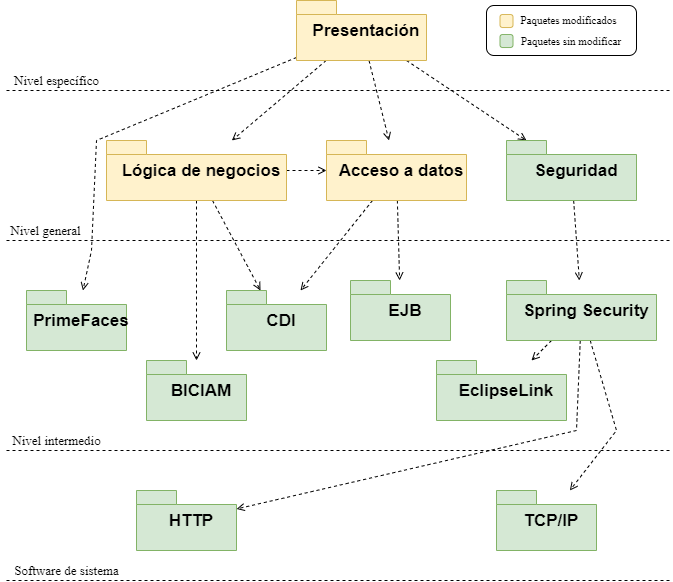
\includegraphics[width=.7\textwidth]{figuras/diagrama-paquetes.png}
	\caption{Diagrama de estructuración en capas basado en reutilización} \label{fig:diagrama-paquetes}
\end{figure}

A continuación se explican aquellos paquetes modificados por el autor:
\begin{description}
	\item[Presentación:] Paquete que contiene las páginas XHTML (\textit{Facelets}) y las plantillas (\textit{Templates}) correspondientes a las mismas.
	\item[Lógica de Negocio:] Paquete que contiene las clases que implementan la lógica del negocio. Este paquete agrupa los controladores, objetos java planos (\textit{POJO} por sus siglas en inglés) útiles, y las clases relacionadas con la solución al modelo de formación de múltiples equipos con la biblioteca BICIAM. 
	\item[Acceso a Datos:] Paquete que contiene las clases para el acceso a datos. Dentro de este se encuentran las \textit{Entity} (clase java con anotaciones, que representa una tabla en la BD), y los modelos (una clase abstracta que define los métodos comunes de creación, actualización y eliminación, y una implementación de esta clase por cada \textit{Entity}) 
\end{description}

\section{Validación del proceso de importación propuesto}
En esta sección se comprueba el correcto funcionamiento de las nuevas funcionalidades incorporadas a la herramienta TEAMSOFT$^+$ vinculadas con el proceso de importación de personas. En la Figura \ref{fig:diagrama-flujo-importar} se presenta el diagrama de flujo asociado a este proceso. 

\begin{figure}[H]
	\centering
	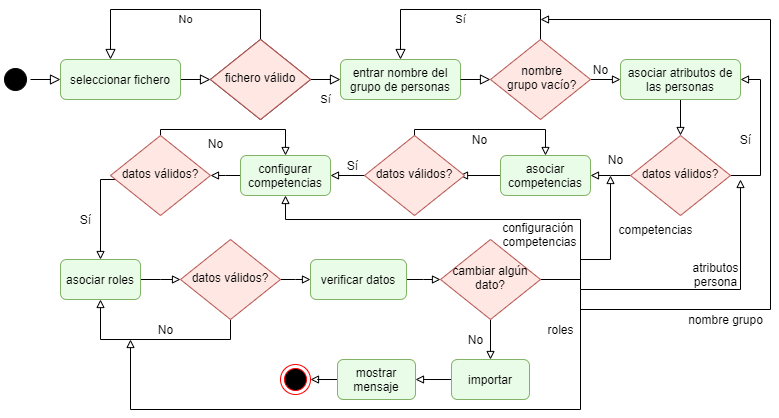
\includegraphics[width=\textwidth]{figuras/diagramas-teamsoft-Flujo-Importar.png}
	\caption{Diagrama de flujo importar} \label{fig:diagrama-flujo-importar}
\end{figure}

El proceso comienza cuando el usuario \textbf{selecciona un fichero} a importar. Este fichero tiene que cumplir las características que se listan en la Tabla \ref{table:especificaciones-fichero}. Este formato permite que la información almacenada en el fichero se adapte a diferentes tipos de problemas.

\begin{table}[H]
	\centering
	\caption{Especificaciones del fichero a importar}\label{table:especificaciones-fichero}
	\begin{tabular} {l | p{10cm}}
		\toprule
		Formato & Valores separados por comas o \textit{CSV} por sus siglas en inglés (\textit{.csv}) \\ \midrule
		Composición & Cada columna representa un atributo de las personas. Mientras que cada fila representa los valores de las personas en cada atributo. \\ \hline
		Campos obligatorios & La experiencia y el nombre de las personas \\ \hline
		Campos adicionales & Todos los atributos relacionados con el problema en cuestión \\ \hline 
		Restricciones & El tipo de dato de cada columna tiene que ser homogéneo \\ \bottomrule
	\end{tabular}
\end{table}

En el paso entrar nombre del grupo de personas el usuario selecciona de los grupos disponibles, a cuál de ellos incorporar las personas a importar. En caso de no existir el grupo deseado, este se crea al finalizar el proceso, justo antes de insertar a las personas. A continuación es necesario asociar las características de las personas disponibles en el fichero de entrada a los atributos de las personas definidos, para esto deben coincidir los tipos de datos. De forma similar, se definen los atributos del fichero a partir de los cuáles se calculan los valores de las competencias utilizando las ecuaciones definidas en las secciones \ref{sec:tran_pel} y \ref{sec:tran_docencia}. En el siguiente paso es necesario establecer los pesos asociados a cada una de las categorías de las competencias. Existen diferentes criterios para determinar estos pesos, en función del tipo de dato de los atributos en el fichero de entrada que influyen en la competencia definidos en el paso anterior. Antes de finalizar el proceso, se mapean los atributos del fichero con los roles correspondientes. En este momento es posible comprobar las configuraciones realizadas, y decidir entonces finalizar el proceso de importación o modificar alguno de los pasos anteriores. \\
A continuación se ejemplifican los pasos anteriores para los casos de los problemas de béisbol y docencia abordados en el presente trabajo.

\subsection{Importación de los datos de los docentes}
A continuación se describe el proceso de importación para el caso específico del problema de la docencia. Para iniciar este proceso se seleccionó el fichero que se muestra en el Anexo \ref{fig:fichero-docencia}. La Tabla \ref{table:importar-fichero-docencia} describe brevemente su contenido.

\begin{table}[H]
	\centering
	\caption{Explicación contenido fichero docencia}\label{table:importar-fichero-docencia}
	\begin{tabular} {l | p{10cm}}
		\toprule
		\textbf{Atributo} & \textbf{Descripción} \\ \midrule
		nombre & Nombre de los profesores \\ \hline
		exp & Años de experiencia laboral de los profesores \\ \hline
		cd & Categoría docente \\ \hline
		cc & Categoría científica \\ \hline
		trabdoc & Evaluación del profesor en el trabajo docente \\ \hline
		trabmet & Evaluación del profesor en el trabajo metodológico\\ \hline
		trabinv & Evaluación del profesor en el trabajo investigativo\\ \hline
		conf & Experiencia del profesor trabajando en el rol de conferencia\\ \hline
		cpractica & Experiencia del profesor trabajando en el rol de clase práctica \\ \hline
		seminario & Experiencia del profesor trabajando en el rol de seminario\\ \hline\\
		lab & Experiencia del profesor trabajando en el rol de Laboratorio\\ \hline\\
		tall & Experiencia del profesor trabajando en el rol de taller \\ \hline\\
		jefeasig & Experiencia del profesor trabajando en el rol de Líder\\ \bottomrule
	\end{tabular}
\end{table}

En este caso el fichero contiene a los profesores (para un total de 16) del departamento de Inteligencia Computacional de la Facultad de Ingeniería Informática. Posteriormente se procede a selecciona como grupo de personas \textbf{profesores IC}. Este grupo no existía con antelación, por lo que se creará al iniciar la importación de las personas. El Anexo \ref{fig:cargar-fichero-docencia} muestra cómo queda la pantalla después de lo explicado. Como siguiente paso, se realiza el mapeo entre los atributos del fichero y las características de las personas. Para esto, se seleccionan los atributos del fichero: \textbf{nombre}, \textbf{exp} y se relacionan con \textbf{Nombre} y \textbf{Experiencia} correspondientemente (ver Anexo \ref{fig:mapeo_atr_pers_doc}). Después, se procede a asociar los atributos del fichero con las competencias y, realizar la configuración correspondiente (ver Anexos \ref{fig:}

\subsection{Importación de los datos de  béisbol}



\section{Generación de soluciones a los problemas de docencia y béisbol}

\subsection{Solución al problema de docencia}

\subsection{Solución al problema de  béisbol}




